\selectlanguage{italian}
\chapter{DAGs}
Nel 2000 J. Pearl ha introdotto un chiaro e innovativo approccio grafico al tema della 
causalità: \textit{Directed Acyclic Graphs}.
L’obiettivo di un DAG è quello di disegnare un sistema causale per rappresentare 
esplicitamente tutte le cause dell’outcome d'interesse.
Il modello di causalità è semplificato in quanto: 
\begin{itemize}
    \item Assume un effetto omogeneo su tutte le osservazioni
    \item Utilizza solo outcome osservabili e non potenziali
    \item Si concentra sull'effetto medio incondizionato del trattamento
    \item Non specifica il tipo di relazione tra le variabili
\end{itemize}
Un po' di terminologia riguardante i grafici aciclici orientati: 
\begin{itemize}
    \item Orientato: tutte le relazioni puntano da una causa a un effetto
    \item Aciclico: partendo da un qualunque vertice non possiamo tornare allo stesso
    \item Percorso: una qualsiasi sequenza di vertici orientati in una qualsiasi direzione
    \item Percorso diretto (o causale): un percorso in cui tutti i nodi puntano in una sola 
        direzione
\end{itemize}
Vengono inoltre detti: 
\begin{itemize}
    \item Genitore: una causa diretta di una variabile
    \item Figlio: l'effetto diretto di una certa variabile
    \item Antenato: una causa diretta o indiretta di una certa variabile
    \item Discendente: un effetto diretto o indiretto di una certa variabile
\end{itemize}
\subsection{DAG - Modello di Markov}
\begin{marginfigure}
    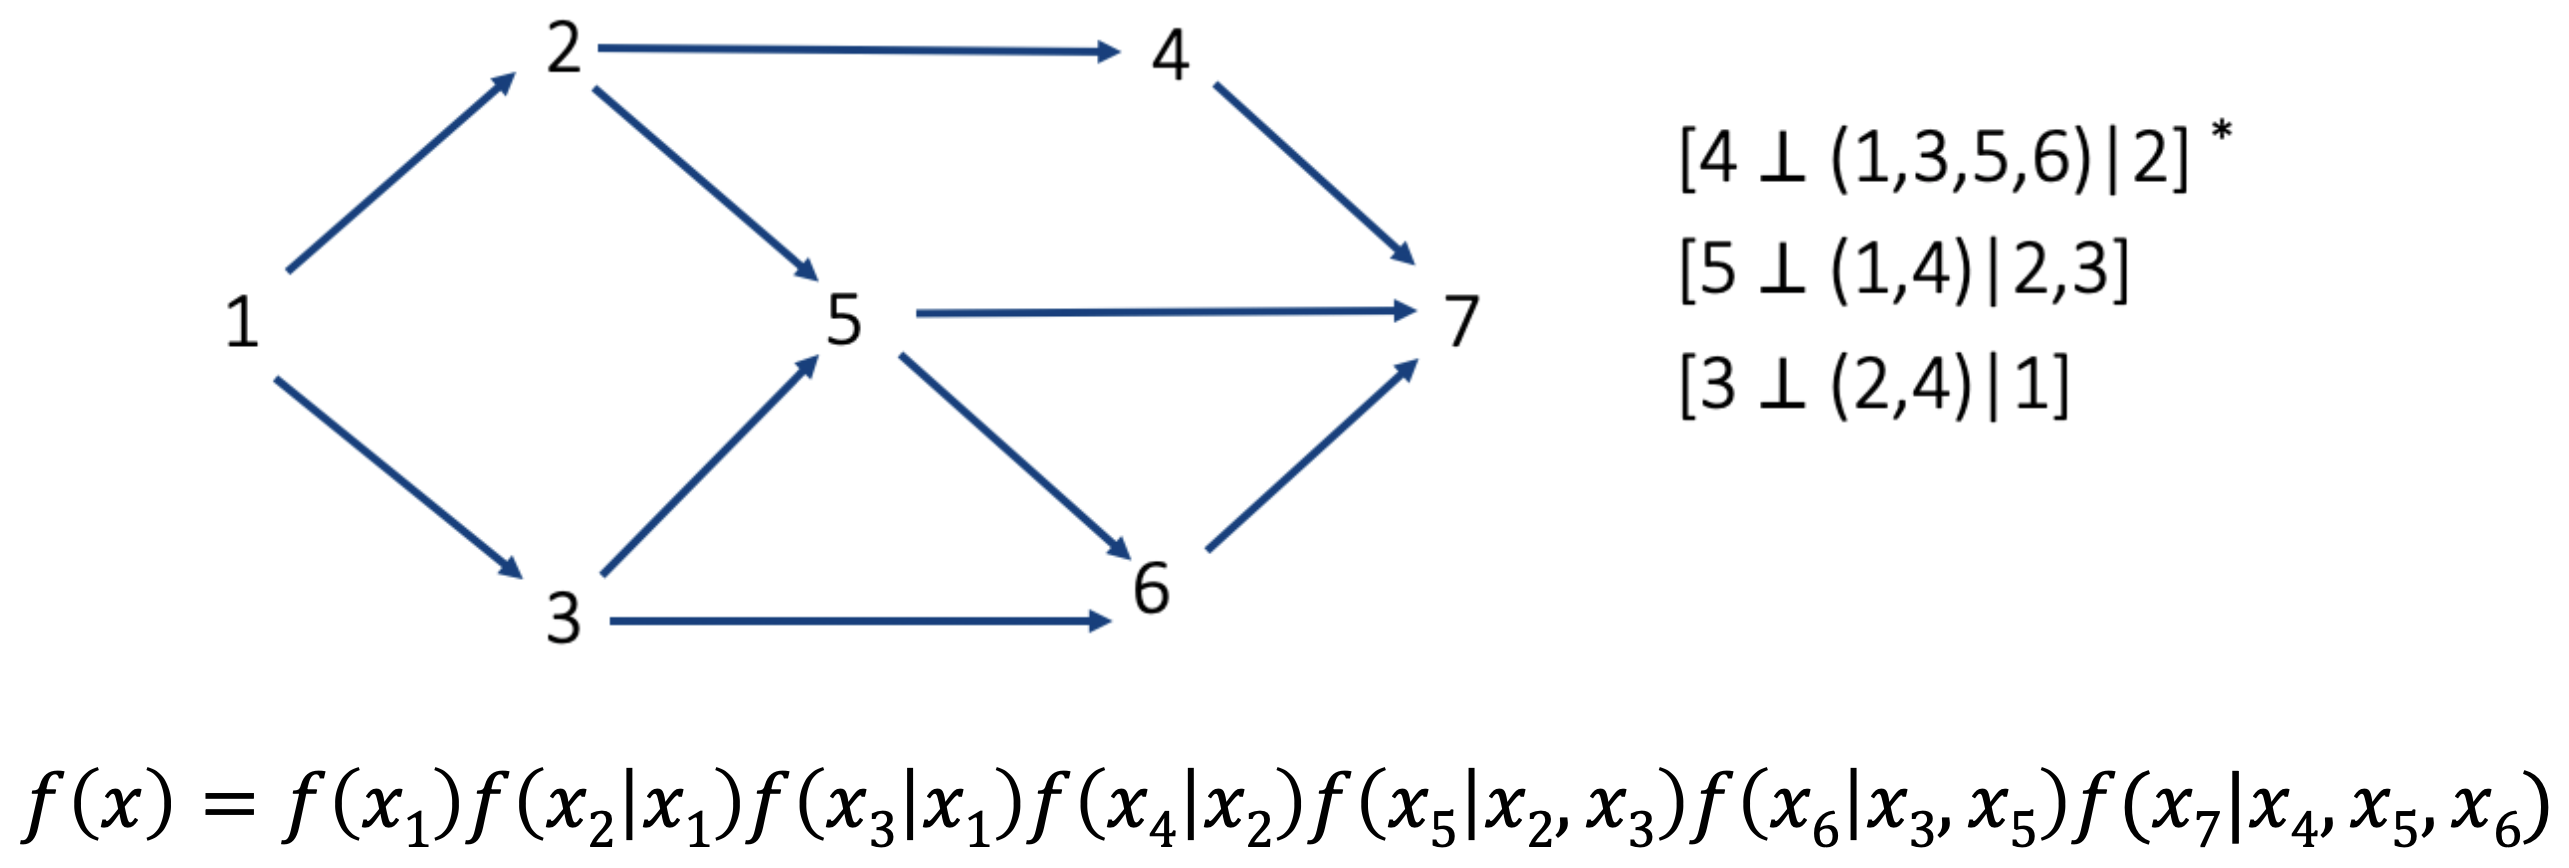
\includegraphics[width = \textwidth]{dag}
\end{marginfigure}
Un DAG è un modello in cui le variabili dipendono solo dai propri genitori e sono 
indipendenti dalle altre variabili. 
La funzione di probabilità di massa è 
\begin{equation}
    f(x) = \Pi_{i = 1}^N f(x_i|x_{iPA})
\end{equation}
\\Se la relazione tra A e B è mediata da C, C è detto mediator\\
Se A e B concausano C, C è un collider\\
Se A e B sono causati da C, C è un cofounder\\
Attenzione perché il cofounder è esattamente ciò che crea problemi nell'analisi: infatti è 
facile confondere la correlazione tra A e B per causalità, mentre la causa della correlazione
è C.
Un percorso causale può essere immediato $A \to B$ o mediato, come per esempio $A \to B \to C$.
L'effetto totale di A su B è la combinazione di tutti i percorsi immediati e mediati da A a B.

L'utilizzo dei DAG permette di offrire una rappresentazione delle relazioni causali,
chiarire le domande di ricerca ed evidenziare i concetti rilevanti, rendere esplicite le 
assunzioni dei nostri modelli, indentificare appropriatamente le variabili da inserire nell’analisi
e ottenere risultati più affidabili, riducendo possibili bias.
Per costruire un DAG: 
\begin{itemize}
    \item Articolare la domanda di ricerca identificando la causa e l’effetto a cui si è 
        interessati («qual è l’effetto di A su B?»)
    \item Identificare altre variabili rilevanti per la relazione, come collider e mediator
    \item Identificare variabili cofounder
    \item Identificare eventuali variabili non misurate o non misurabili
    \item Identificare possibili processi di selezione nello studio
\end{itemize}
Negli anni sono stati creati strumenti a supporto della costruzione di un DAG come 
\url{http://www.dagitty.net/}
\vspace{0.5cm}

\large Paradosso di Simpson
\normalsize
\\Situazione statistica nella quale un trend o una relazione che è osservata tra diversi 
sottogruppi sparisce quando i gruppi sono combinati. In altre parole, dividendo i dati in 
gruppi, le conclusioni sono diverse rispetto a quelle derivanti da un’analisi aggregata.
